\documentclass{article}
\usepackage[utf8]{inputenc}
\usepackage{hyperref}
\usepackage{listings}
\usepackage{xcolor}

\definecolor{codegreen}{rgb}{0,0.6,0}
\definecolor{codegray}{rgb}{0.5,0.5,0.5}
\definecolor{codepurple}{rgb}{0.58,0,0.82}
\definecolor{backcolour}{rgb}{0.95,0.95,0.92}

\lstdefinestyle{mystyle}{
    backgroundcolor=\color{backcolour},   
    commentstyle=\color{codegreen},
    keywordstyle=\color{magenta},
    numberstyle=\tiny\color{codegray},
    stringstyle=\color{codepurple},
    basicstyle=\ttfamily\footnotesize,
    breakatwhitespace=false,         
    breaklines=true,                 
    captionpos=b,                    
    keepspaces=true,                 
    numbers=left,                    
    numbersep=5pt,                  
    showspaces=false,                
    showstringspaces=false,
    showtabs=false,                  
    tabsize=2
}

\lstset{style=mystyle}
\hypersetup{
    colorlinks=true,
    linkcolor=blue,
    filecolor=magenta,      
    urlcolor=cyan,
    pdftitle={Overleaf Example},
    pdfpagemode=FullScreen,
    }

\author{Tarushii Goel}
\date{2020}

\usepackage[letterpaper, margin=1in]{geometry}
\usepackage{natbib}
\usepackage{graphicx}
\usepackage{amsmath}



\begin{document}

\begin{center}
\fbox{\fbox{\parbox{5.5in}{\centering
Problem Set: Pytorch \\
Due date:  10/13/21\\
Total Points: 15\\
Send your code and writeup to tjmachinelearning@gmail.com}}}
\end{center}
 
\vspace{5mm}
 
\makebox[\textwidth]{Name and Grade:\enspace\hrulefill}
 
\vspace{5mm}

\begin{enumerate}
	\item (10 points) Using what you learned about Pytorch in the lecture, as well as your own exploration of the torch.nn and torch.optim modules, train a CNN to classify objects in the CIFAR-10 dataset. Attach a copy of your code as well as a short reflection in your email. Guiding Questions: What did you learn about Pytorch through this exercise? What architecture did you use? What was your accuracy? What steps did you take to increase the accuracy? How long did you need to train? Did you perform and image preprocessing or data augmentation, and if you did, how did that affect accuracies? \\ 
	\pagebreak
	\item (5 points) Replicate these two CNN architectures and train them on the CIFAR-10 Dataset (you will need to change input/output layer dimensions slightly, do this as you like but don't change the architecture significantly). How do the accuracies compare? Why do you think that is? Attach your code and writeup in the email. 
\begin{center}
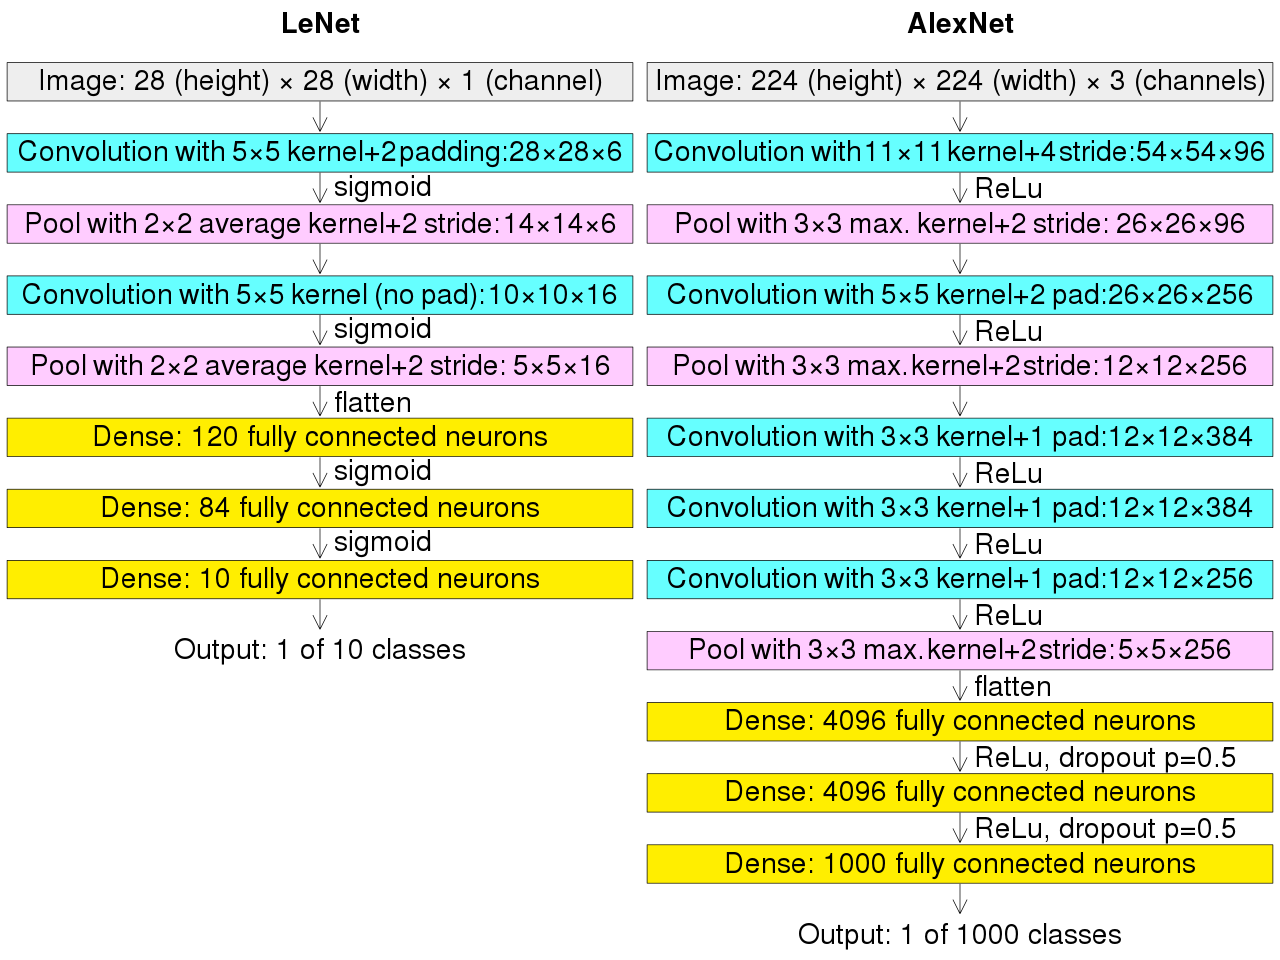
\includegraphics[scale=0.3]{networks.svg}
\end{center}

\end {enumerate}
\end{document}
